\documentclass[12pt, titlepage]{article}
\usepackage{graphicx}
\usepackage{booktabs}
\usepackage{tabularx}
\usepackage{hyperref}
\hypersetup{
    colorlinks,
    citecolor=black,
    filecolor=black,
    linkcolor=red,
    urlcolor=blue
}
\usepackage[round]{natbib}

%% Comments

\usepackage{color}

\newif\ifcomments\commentstrue %displays comments
%\newif\ifcomments\commentsfalse %so that comments do not display

\ifcomments
\newcommand{\authornote}[3]{\textcolor{#1}{[#3 ---#2]}}
\newcommand{\todo}[1]{\textcolor{red}{[TODO: #1]}}
\else
\newcommand{\authornote}[3]{}
\newcommand{\todo}[1]{}
\fi

\newcommand{\wss}[1]{\authornote{blue}{SS}{#1}} 
\newcommand{\plt}[1]{\authornote{magenta}{TPLT}{#1}} %For explanation of the template
\newcommand{\an}[1]{\authornote{cyan}{Author}{#1}}

%% Common Parts

\newcommand{\progname}{ProgName} % PUT YOUR PROGRAM NAME HERE
\newcommand{\authname}{Team \#, Team Name
\\ Student 1 name
\\ Student 2 name
\\ Student 3 name
\\ Student 4 name} % AUTHOR NAMES                  

\usepackage{hyperref}
    \hypersetup{colorlinks=true, linkcolor=blue, citecolor=blue, filecolor=blue,
                urlcolor=blue, unicode=false}
    \urlstyle{same}
                                


\begin{document}

\title{Verification and Validation Report for Centrality In Graphs} 
\author{Atiyeh Sayadi}
\date{\today}
	
\maketitle

\pagenumbering{roman}

\section{Revision History}

\begin{tabularx}{\textwidth}{p{3cm}p{2cm}X}
\toprule {\bf Date} & {\bf Version} & {\bf Notes}\\
\midrule
April 10, 2024 & Notes\\
\bottomrule
\end{tabularx}

~\newpage

\section{Symbols, Abbreviations and Acronyms}

\renewcommand{\arraystretch}{1.2}
\begin{tabular}{l l} 
  \toprule		
  \textbf{symbol} & \textbf{description}\\
  \midrule 
  T & Test\\
  \bottomrule
\end{tabular}\\



\newpage

\tableofcontents

\listoftables %if appropriate

\listoffigures %if appropriate

\newpage

\pagenumbering{arabic}


This document provides a summary of the tests conducted for the centrality project in graphs.

\section{Functional Requirements Evaluation}
This section tests the functional requirements of the system, the description of which is as follows:
\begin{enumerate}
\item{Test1: Bound Testing for degree centrality\\}	
Based on requirements 1 and 2 of this project, it is necessary for the degree centrality to be accurately calculated for all nodes. We know that this metric for each node is between zero and one. Therefore, a function needs to be written to evaluate this value for each node based on the allowable range and report any discrepancies found.
\item{Test2: Bound Testing for closeness centrality\\}
Based on requirements 3 and 4 of this project, it is necessary for the closeness centrality to be accurately calculated for all nodes. We know that this metric for each node is between zero and one. Therefore, a function needs to be written to evaluate this value for each node based on the allowable range and report any discrepancies found.

\end{enumerate}

The implementation of both tests is available in the  (\href{https://github.com/AtiyehSayadi/Centrality-In-Graphs/blob/main/test/test_cig.py}{test\_cig}).
\section{Nonfunctional Requirements Evaluation}

\subsection{Usability}
No user feedback has been obtained for this test.		
\subsection{maintainability}
\begin{enumerate}

\item{Test3: Code Testing\\}
By utilizing the Python's Pylint tool, the codes can be standardized, ensuring high maintainability.
\end{enumerate}
\subsection{Accuracy}
\begin{enumerate}
\item{Test4: Correctness Testing for DC\\}

 Using the NetworkX library functions in Python, the centrality of each node is calculated for the given graph, and it is compared with the output of the program(Based on requirements 1 and 2).

How test will be performed: Nodes for which the calculated centrality differs from the library function output are displayed.

\item{Test5: Correctness Testing for CC\\}

Using the NetworkX library functions in Python, the centrality of each node is calculated for the given graph, and it is compared with the output of the program(Based on requirements 3 and 4).

How test will be performed: Nodes for which the calculated centrality differs from the library function output are displayed.

\end{enumerate}
The implementation of both tests is available in the  (\href{https://github.com/AtiyehSayadi/Centrality-In-Graphs/blob/main/test/test\_cig.py}{test\_cig}).
\section{Comparison to Existing Implementation}	
Previously, the plan was to implement the main graph of the project in the form of an adjacency matrix, representing the relationships between nodes, or the adjacency matrix, and related concepts. However, following feedback from Dr. Spencer Smith, it was decided to design this project in a modular manner based on the abstract data type, which is the graph itself. This modular design approach significantly enhances usability and maintainability.

\section{Unit Testing}
The implementation of these tests is available in the  (\href{https://github.com/AtiyehSayadi/Centrality-In-Graphs/blob/main/test/test\_graph.py}{test\_graph}).
\begin{figure}[h!]
    \centering
   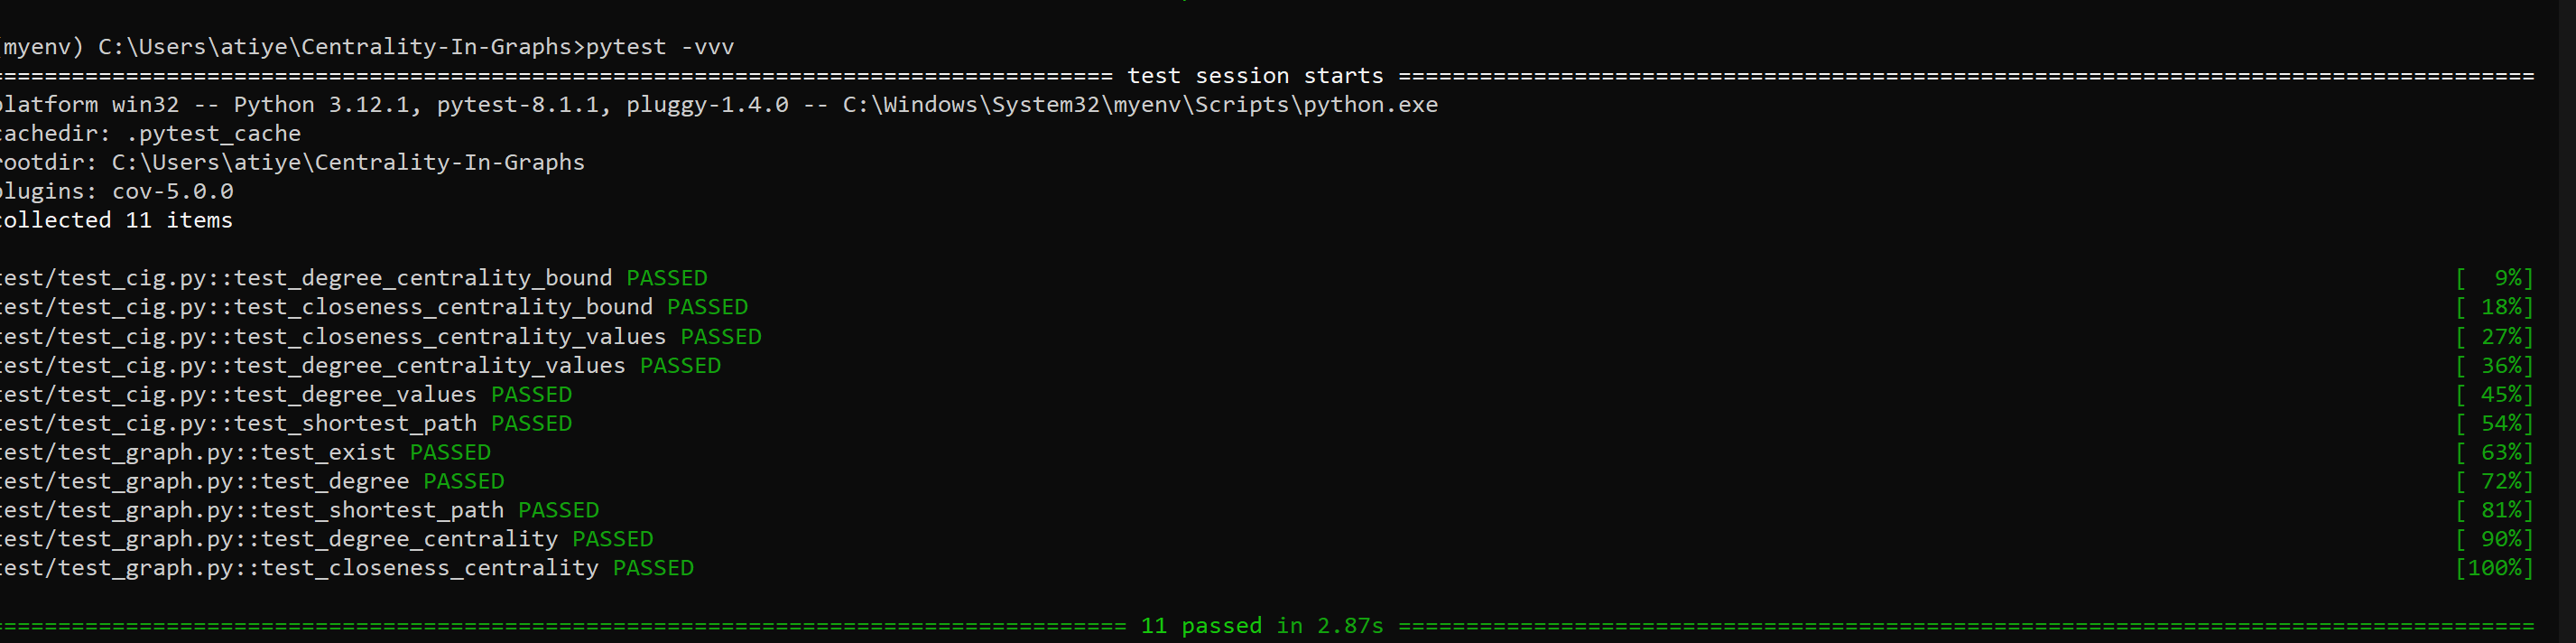
\includegraphics[width=1.0\textwidth, keepaspectratio]{repo.png}
    \caption{Test logs}
\end{figure}
\section{Changes Due to Testing}
After numerous reviews, this code has undergone several changes, including the definition of the graph data type and the class related to graph implementation. Additionally, the method for displaying output to highlight important nodes has been modified per Dr. Spencer Smith's directive.


\section{Automated Testing}

All tests have been automated using Python's testing framework (Pytest) and linting tool (Pylint).		
\section{Trace to Requirements}
\begin{table}[h!]
\centering
\begin{tabular}{|c|p{0.5cm}|p{0.5cm}|p{0.5cm}|p{0.5cm}|p{1cm}|p{1cm}|p{1cm}|p{1cm}|}
\hline
	&FR1 &FR2 & FR3 & FR4 &NFR1 &NFR2 & NFR3 & NFR4\\
\hline
 Bound Testing for degree centrality     & X& X&  &  & X & & & \\ \hline
Bound Testing for closeness centrality    & &   &  X&X  & X & & & \\ \hline
Code Testing    &   &   &  &  & X & & X& \\ \hline
Correctness Testing for DC\    &X  &X   &  &  & X & & & \\ \hline
Correctness Testing for CC    &  &  & X & X &  & & & \\ \hline
test\_degree\_centrality    & X & X &  &  &  & & & \\ \hline
 test\_closeness\_centrality    &  &  & X & X &  & & & \\ \hline
test\_exist    & X &X  & X & X &  & & & \\ \hline
test\_degree    & X &X  &  &  &  & & & \\ \hline
test\_shortest\_path    &  &  & X & X &  & & & \\ \hline
\end{tabular}
\caption{Trace to Requirements}
\label{Table:A_trace}
\end{table}		
\section{Trace to Modules}		
\begin{table}[h!]
\centering
\begin{tabular}{|c|c|c|c|c|c|c|c|c|c|c|c|c|c|c|c|c|c|c|c|}
\hline
	&File &Graph & ShowGraph \\
\hline
 Bound Testing for degree centrality     & & X& \\ \hline
Bound Testing for closeness centrality    & &  X&  \\ \hline
Code Testing    &  X & X  & X \\ \hline
Correctness Testing for DC\    & &X   & X\\ \hline
Correctness Testing for CC    &  &  X& X \\ \hline
test\_degree\_centrality    &  & X &   \\ \hline
 test\_closeness\_centrality    &  &  X& \\ \hline
test\_exist    &  &X  &  \\ \hline
test\_degree    & &X  &  \\ \hline
test\_shortest\_path    &X  &  & \\ \hline
\end{tabular}
\label{Table:A_trace}
\caption{Trace to Modules}
\end{table}	
\newpage
\section{Code Coverage Metrics}
\begin{figure}[h!]
    \centering
   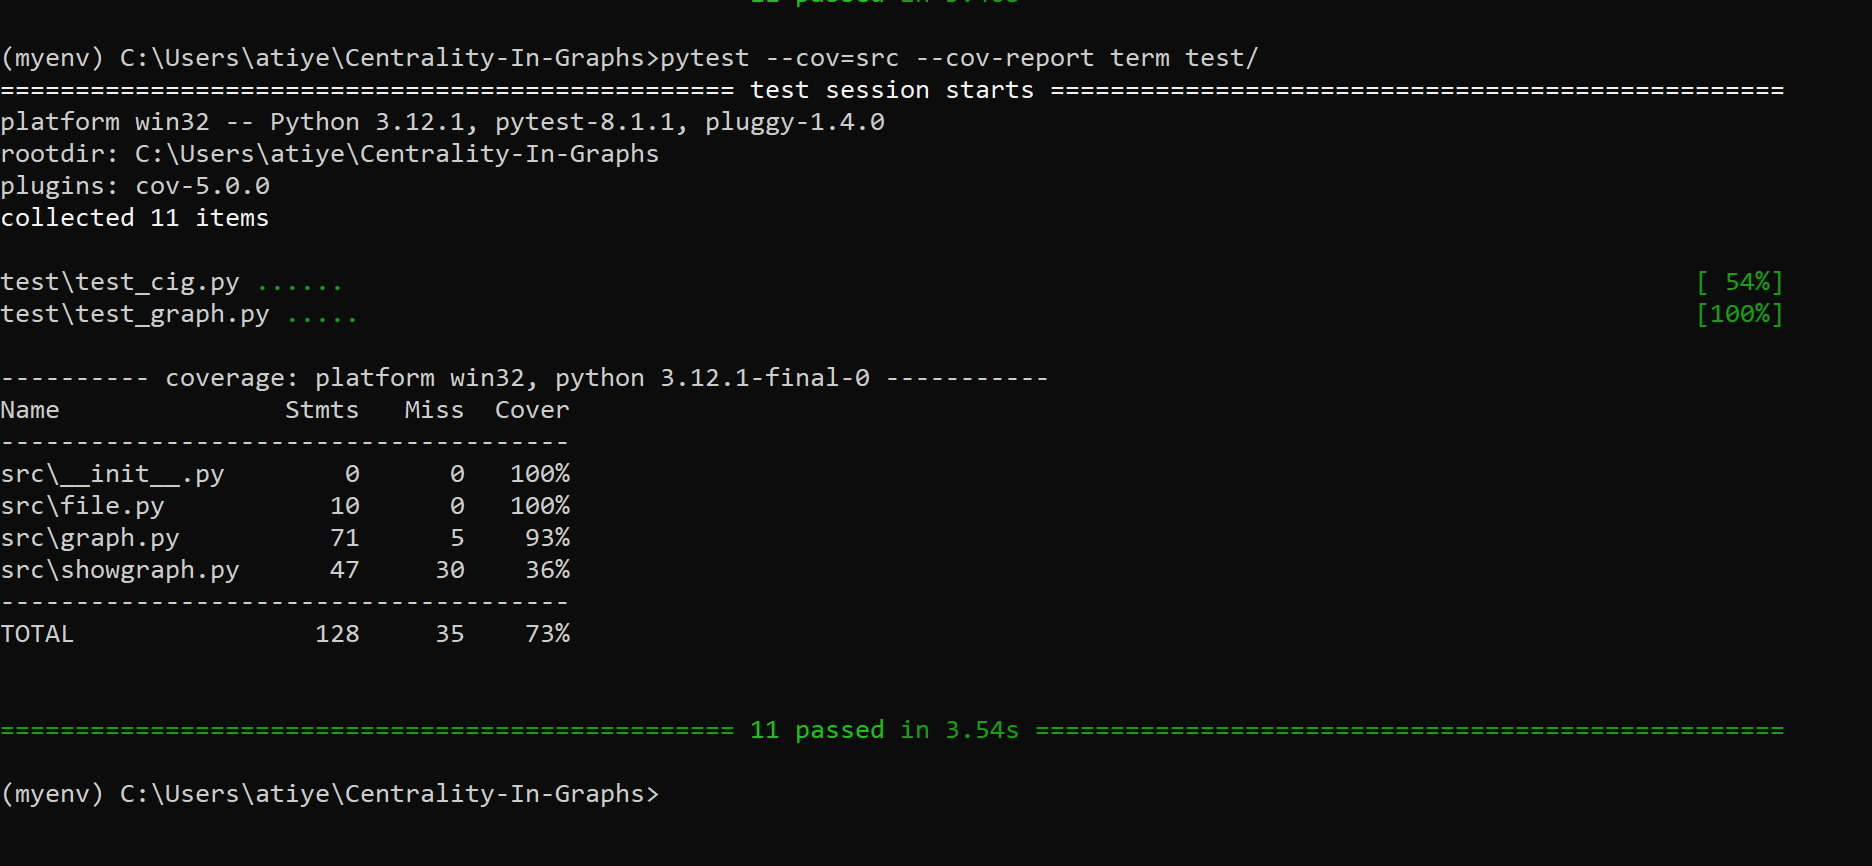
\includegraphics[width=1.0\textwidth, keepaspectratio]{cov.png}
    \caption{Code Coverage Metrics}
\end{figure}

\bibliographystyle{plainnat}


\newpage{}



\end{document}